% GNUPLOT: LaTeX picture with Postscript
\begingroup
  \makeatletter
  \providecommand\color[2][]{%
    \GenericError{(gnuplot) \space\space\space\@spaces}{%
      Package color not loaded in conjunction with
      terminal option `colourtext'%
    }{See the gnuplot documentation for explanation.%
    }{Either use 'blacktext' in gnuplot or load the package
      color.sty in LaTeX.}%
    \renewcommand\color[2][]{}%
  }%
  \providecommand\includegraphics[2][]{%
    \GenericError{(gnuplot) \space\space\space\@spaces}{%
      Package graphicx or graphics not loaded%
    }{See the gnuplot documentation for explanation.%
    }{The gnuplot epslatex terminal needs graphicx.sty or graphics.sty.}%
    \renewcommand\includegraphics[2][]{}%
  }%
  \providecommand\rotatebox[2]{#2}%
  \@ifundefined{ifGPcolor}{%
    \newif\ifGPcolor
    \GPcolortrue
  }{}%
  \@ifundefined{ifGPblacktext}{%
    \newif\ifGPblacktext
    \GPblacktexttrue
  }{}%
  % define a \g@addto@macro without @ in the name:
  \let\gplgaddtomacro\g@addto@macro
  % define empty templates for all commands taking text:
  \gdef\gplbacktext{}%
  \gdef\gplfronttext{}%
  \makeatother
  \ifGPblacktext
    % no textcolor at all
    \def\colorrgb#1{}%
    \def\colorgray#1{}%
  \else
    % gray or color?
    \ifGPcolor
      \def\colorrgb#1{\color[rgb]{#1}}%
      \def\colorgray#1{\color[gray]{#1}}%
      \expandafter\def\csname LTw\endcsname{\color{white}}%
      \expandafter\def\csname LTb\endcsname{\color{black}}%
      \expandafter\def\csname LTa\endcsname{\color{black}}%
      \expandafter\def\csname LT0\endcsname{\color[rgb]{1,0,0}}%
      \expandafter\def\csname LT1\endcsname{\color[rgb]{0,1,0}}%
      \expandafter\def\csname LT2\endcsname{\color[rgb]{0,0,1}}%
      \expandafter\def\csname LT3\endcsname{\color[rgb]{1,0,1}}%
      \expandafter\def\csname LT4\endcsname{\color[rgb]{0,1,1}}%
      \expandafter\def\csname LT5\endcsname{\color[rgb]{1,1,0}}%
      \expandafter\def\csname LT6\endcsname{\color[rgb]{0,0,0}}%
      \expandafter\def\csname LT7\endcsname{\color[rgb]{1,0.3,0}}%
      \expandafter\def\csname LT8\endcsname{\color[rgb]{0.5,0.5,0.5}}%
    \else
      % gray
      \def\colorrgb#1{\color{black}}%
      \def\colorgray#1{\color[gray]{#1}}%
      \expandafter\def\csname LTw\endcsname{\color{white}}%
      \expandafter\def\csname LTb\endcsname{\color{black}}%
      \expandafter\def\csname LTa\endcsname{\color{black}}%
      \expandafter\def\csname LT0\endcsname{\color{black}}%
      \expandafter\def\csname LT1\endcsname{\color{black}}%
      \expandafter\def\csname LT2\endcsname{\color{black}}%
      \expandafter\def\csname LT3\endcsname{\color{black}}%
      \expandafter\def\csname LT4\endcsname{\color{black}}%
      \expandafter\def\csname LT5\endcsname{\color{black}}%
      \expandafter\def\csname LT6\endcsname{\color{black}}%
      \expandafter\def\csname LT7\endcsname{\color{black}}%
      \expandafter\def\csname LT8\endcsname{\color{black}}%
    \fi
  \fi
    \setlength{\unitlength}{0.0500bp}%
    \ifx\gptboxheight\undefined%
      \newlength{\gptboxheight}%
      \newlength{\gptboxwidth}%
      \newsavebox{\gptboxtext}%
    \fi%
    \setlength{\fboxrule}{0.5pt}%
    \setlength{\fboxsep}{1pt}%
    \definecolor{tbcol}{rgb}{1,1,1}%
\begin{picture}(4520.00,4240.00)%
    \gplgaddtomacro\gplbacktext{%
    }%
    \gplgaddtomacro\gplfronttext{%
      \csname LTb\endcsname%%
      \put(577,2476){\makebox(0,0)[r]{\strut{}$-160$}}%
      \csname LTb\endcsname%%
      \put(577,2662){\makebox(0,0)[r]{\strut{}$-120$}}%
      \csname LTb\endcsname%%
      \put(577,2847){\makebox(0,0)[r]{\strut{}$-80$}}%
      \csname LTb\endcsname%%
      \put(577,3032){\makebox(0,0)[r]{\strut{}$-40$}}%
      \csname LTb\endcsname%%
      \put(577,3217){\makebox(0,0)[r]{\strut{}$0$}}%
      \csname LTb\endcsname%%
      \put(577,3402){\makebox(0,0)[r]{\strut{}$40$}}%
      \csname LTb\endcsname%%
      \put(577,3588){\makebox(0,0)[r]{\strut{}$80$}}%
      \csname LTb\endcsname%%
      \put(577,3773){\makebox(0,0)[r]{\strut{}$120$}}%
      \csname LTb\endcsname%%
      \put(577,3958){\makebox(0,0)[r]{\strut{}$160$}}%
      \csname LTb\endcsname%%
      \put(675,2208){\makebox(0,0){\strut{}}}%
      \csname LTb\endcsname%%
      \put(952,2208){\makebox(0,0){\strut{}}}%
      \csname LTb\endcsname%%
      \put(1230,2208){\makebox(0,0){\strut{}}}%
      \csname LTb\endcsname%%
      \put(1508,2208){\makebox(0,0){\strut{}}}%
      \csname LTb\endcsname%%
      \put(1786,2208){\makebox(0,0){\strut{}}}%
      \csname LTb\endcsname%%
      \put(2064,2208){\makebox(0,0){\strut{}}}%
      \csname LTb\endcsname%%
      \put(2341,2208){\makebox(0,0){\strut{}}}%
      \csname LTb\endcsname%%
      \put(219,3217){\rotatebox{-270.00}{\makebox(0,0){\normalsize $\Psi$}}}%
      \csname LTb\endcsname%%
      \put(1323,3336){\rotatebox{-66.00}{\makebox(0,0){\strut{}\textcolor{black}{\footnotesize 500}}}}%
      \csname LTb\endcsname%%
      \put(1665,3266){\rotatebox{130.00}{\makebox(0,0){\strut{}\textcolor{black}{\footnotesize 400}}}}%
      \csname LTb\endcsname%%
      \put(1347,3139){\rotatebox{-27.00}{\makebox(0,0){\strut{}\textcolor{black}{\footnotesize 400}}}}%
      \csname LTb\endcsname%%
      \put(1417,3544){\rotatebox{154.00}{\makebox(0,0){\strut{}\textcolor{black}{\footnotesize 300}}}}%
      \csname LTb\endcsname%%
      \put(1412,3014){\rotatebox{-39.00}{\makebox(0,0){\strut{}\textcolor{black}{\footnotesize 300}}}}%
      \csname LTb\endcsname%%
      \put(1865,3179){\rotatebox{113.00}{\makebox(0,0){\strut{}\textcolor{black}{\footnotesize 200}}}}%
      \csname LTb\endcsname%%
      \put(1064,3700){\rotatebox{-143.00}{\makebox(0,0){\strut{}\textcolor{black}{\footnotesize 200}}}}%
      \csname LTb\endcsname%%
      \put(1501,2870){\rotatebox{-26.00}{\makebox(0,0){\strut{}\textcolor{black}{\footnotesize 200}}}}%
      \csname LTb\endcsname%%
      \put(963,3785){\rotatebox{39.00}{\makebox(0,0){\strut{}\textcolor{black}{\footnotesize 100}}}}%
      \csname LTb\endcsname%%
      \put(1795,3791){\rotatebox{42.00}{\makebox(0,0){\strut{}\textcolor{black}{\footnotesize 100}}}}%
      \csname LTb\endcsname%%
      \put(1921,3220){\rotatebox{-71.00}{\makebox(0,0){\strut{}\textcolor{black}{\footnotesize 100}}}}%
      \csname LTb\endcsname%%
      \put(995,3448){\rotatebox{-43.00}{\makebox(0,0){\strut{}\textcolor{black}{\footnotesize 100}}}}%
      \csname LTb\endcsname%%
      \put(1025,2669){\rotatebox{-33.00}{\makebox(0,0){\strut{}\textcolor{black}{\footnotesize 100}}}}%
      \csname LTb\endcsname%%
      \put(1865,2557){\rotatebox{-28.00}{\makebox(0,0){\strut{}\textcolor{black}{\footnotesize 100}}}}%
      \csname LTb\endcsname%%
      \put(743,3392){\rotatebox{-112.00}{\makebox(0,0){\strut{}\textcolor{black}{\footnotesize 50}}}}%
      \csname LTb\endcsname%%
      \put(2022,3364){\rotatebox{-149.00}{\makebox(0,0){\strut{}\textcolor{black}{\footnotesize 50}}}}%
      \csname LTb\endcsname%%
      \put(1375,3744){\rotatebox{-28.00}{\makebox(0,0){\strut{}\textcolor{black}{\footnotesize 50}}}}%
      \csname LTb\endcsname%%
      \put(1408,2706){\rotatebox{31.00}{\makebox(0,0){\strut{}\textcolor{black}{\footnotesize 50}}}}%
      \csname LTb\endcsname%%
      \put(1508,4174){\makebox(0,0){\strut{}Conformational Energy (meV)}}%
    }%
    \gplgaddtomacro\gplbacktext{%
    }%
    \gplgaddtomacro\gplfronttext{%
      \csname LTb\endcsname%%
      \put(2512,2476){\makebox(0,0)[r]{\strut{}}}%
      \csname LTb\endcsname%%
      \put(2512,2662){\makebox(0,0)[r]{\strut{}}}%
      \csname LTb\endcsname%%
      \put(2512,2847){\makebox(0,0)[r]{\strut{}}}%
      \csname LTb\endcsname%%
      \put(2512,3032){\makebox(0,0)[r]{\strut{}}}%
      \csname LTb\endcsname%%
      \put(2512,3217){\makebox(0,0)[r]{\strut{}}}%
      \csname LTb\endcsname%%
      \put(2512,3402){\makebox(0,0)[r]{\strut{}}}%
      \csname LTb\endcsname%%
      \put(2512,3588){\makebox(0,0)[r]{\strut{}}}%
      \csname LTb\endcsname%%
      \put(2512,3773){\makebox(0,0)[r]{\strut{}}}%
      \csname LTb\endcsname%%
      \put(2512,3958){\makebox(0,0)[r]{\strut{}}}%
      \csname LTb\endcsname%%
      \put(2610,2208){\makebox(0,0){\strut{}}}%
      \csname LTb\endcsname%%
      \put(2887,2208){\makebox(0,0){\strut{}}}%
      \csname LTb\endcsname%%
      \put(3165,2208){\makebox(0,0){\strut{}}}%
      \csname LTb\endcsname%%
      \put(3443,2208){\makebox(0,0){\strut{}}}%
      \csname LTb\endcsname%%
      \put(3721,2208){\makebox(0,0){\strut{}}}%
      \csname LTb\endcsname%%
      \put(3999,2208){\makebox(0,0){\strut{}}}%
      \csname LTb\endcsname%%
      \put(4276,2208){\makebox(0,0){\strut{}}}%
      \csname LTb\endcsname%%
      \put(2635,3628){\rotatebox{37.00}{\makebox(0,0){\strut{}\textcolor{black}{\footnotesize 3.0}}}}%
      \csname LTb\endcsname%%
      \put(4227,3062){\rotatebox{156.00}{\makebox(0,0){\strut{}\textcolor{black}{\footnotesize 3.0}}}}%
      \csname LTb\endcsname%%
      \put(3270,3381){\rotatebox{-78.00}{\makebox(0,0){\strut{}\textcolor{black}{\footnotesize 2.5}}}}%
      \csname LTb\endcsname%%
      \put(2894,3804){\rotatebox{-7.00}{\makebox(0,0){\strut{}\textcolor{black}{\footnotesize 2.5}}}}%
      \csname LTb\endcsname%%
      \put(2793,3247){\rotatebox{-127.00}{\makebox(0,0){\strut{}\textcolor{black}{\footnotesize 2.5}}}}%
      \csname LTb\endcsname%%
      \put(4138,3489){\rotatebox{-88.00}{\makebox(0,0){\strut{}\textcolor{black}{\footnotesize 2.5}}}}%
      \csname LTb\endcsname%%
      \put(3914,2912){\rotatebox{-101.00}{\makebox(0,0){\strut{}\textcolor{black}{\footnotesize 2.5}}}}%
      \csname LTb\endcsname%%
      \put(2831,2987){\rotatebox{91.00}{\makebox(0,0){\strut{}\textcolor{black}{\footnotesize 2.0}}}}%
      \csname LTb\endcsname%%
      \put(3172,3288){\rotatebox{-47.00}{\makebox(0,0){\strut{}\textcolor{black}{\footnotesize 2.0}}}}%
      \csname LTb\endcsname%%
      \put(3557,2853){\rotatebox{-38.00}{\makebox(0,0){\strut{}\textcolor{black}{\footnotesize 2.0}}}}%
      \csname LTb\endcsname%%
      \put(3263,3690){\rotatebox{-101.00}{\makebox(0,0){\strut{}\textcolor{black}{\footnotesize 2.0}}}}%
      \csname LTb\endcsname%%
      \put(3638,3255){\rotatebox{-59.00}{\makebox(0,0){\strut{}\textcolor{black}{\footnotesize 2.0}}}}%
      \csname LTb\endcsname%%
      \put(4029,3305){\rotatebox{64.00}{\makebox(0,0){\strut{}\textcolor{black}{\footnotesize 2.0}}}}%
      \csname LTb\endcsname%%
      \put(2819,2723){\rotatebox{52.00}{\makebox(0,0){\strut{}\textcolor{black}{\footnotesize 1.5}}}}%
      \csname LTb\endcsname%%
      \put(3162,3148){\rotatebox{-17.00}{\makebox(0,0){\strut{}\textcolor{black}{\footnotesize 1.5}}}}%
      \csname LTb\endcsname%%
      \put(3405,2612){\rotatebox{-106.00}{\makebox(0,0){\strut{}\textcolor{black}{\footnotesize 1.5}}}}%
      \csname LTb\endcsname%%
      \put(3732,3935){\rotatebox{-176.00}{\makebox(0,0){\strut{}\textcolor{black}{\footnotesize 1.5}}}}%
      \csname LTb\endcsname%%
      \put(3559,3489){\rotatebox{-45.00}{\makebox(0,0){\strut{}\textcolor{black}{\footnotesize 1.5}}}}%
      \csname LTb\endcsname%%
      \put(3964,3448){\rotatebox{78.00}{\makebox(0,0){\strut{}\textcolor{black}{\footnotesize 1.5}}}}%
      \csname LTb\endcsname%%
      \put(2945,2791){\rotatebox{56.00}{\makebox(0,0){\strut{}\textcolor{black}{\footnotesize 1.0}}}}%
      \csname LTb\endcsname%%
      \put(3280,2636){\rotatebox{-124.00}{\makebox(0,0){\strut{}\textcolor{black}{\footnotesize 1.0}}}}%
      \csname LTb\endcsname%%
      \put(3665,3837){\rotatebox{-162.00}{\makebox(0,0){\strut{}\textcolor{black}{\footnotesize 1.0}}}}%
      \csname LTb\endcsname%%
      \put(3904,3582){\rotatebox{60.00}{\makebox(0,0){\strut{}\textcolor{black}{\footnotesize 1.0}}}}%
      \csname LTb\endcsname%%
      \put(2992,2736){\rotatebox{-132.00}{\makebox(0,0){\strut{}\textcolor{black}{\footnotesize 0.5}}}}%
      \csname LTb\endcsname%%
      \put(3740,3766){\rotatebox{-140.00}{\makebox(0,0){\strut{}\textcolor{black}{\footnotesize 0.5}}}}%
      \csname LTb\endcsname%%
      \put(3443,4174){\makebox(0,0){Dipole Strength (Debye)}}%
    }%
    \gplgaddtomacro\gplbacktext{%
    }%
    \gplgaddtomacro\gplfronttext{%
      \csname LTb\endcsname%%
      \put(577,556){\makebox(0,0)[r]{\strut{}$-160$}}%
      \csname LTb\endcsname%%
      \put(577,742){\makebox(0,0)[r]{\strut{}$-120$}}%
      \csname LTb\endcsname%%
      \put(577,927){\makebox(0,0)[r]{\strut{}$-80$}}%
      \csname LTb\endcsname%%
      \put(577,1112){\makebox(0,0)[r]{\strut{}$-40$}}%
      \csname LTb\endcsname%%
      \put(577,1297){\makebox(0,0)[r]{\strut{}$0$}}%
      \csname LTb\endcsname%%
      \put(577,1482){\makebox(0,0)[r]{\strut{}$40$}}%
      \csname LTb\endcsname%%
      \put(577,1668){\makebox(0,0)[r]{\strut{}$80$}}%
      \csname LTb\endcsname%%
      \put(577,1853){\makebox(0,0)[r]{\strut{}$120$}}%
      \csname LTb\endcsname%%
      \put(577,2038){\makebox(0,0)[r]{\strut{}$160$}}%
      \csname LTb\endcsname%%
      \put(767,288){\makebox(0,0){\strut{}$-160$}}%
      \csname LTb\endcsname%%
      \put(1138,288){\makebox(0,0){\strut{}$-80$}}%
      \csname LTb\endcsname%%
      \put(1508,288){\makebox(0,0){\strut{}$0$}}%
      \csname LTb\endcsname%%
      \put(1878,288){\makebox(0,0){\strut{}$80$}}%
      \csname LTb\endcsname%%
      \put(2249,288){\makebox(0,0){\strut{}$160$}}%
      \csname LTb\endcsname%%
      \put(219,1297){\rotatebox{-270.00}{\makebox(0,0){\normalsize $\Psi$}}}%
      \csname LTb\endcsname%%
      \put(1508,24){\makebox(0,0){\normalsize $\Phi$}}%
      \csname LTb\endcsname%%
      \put(1449,1402){\rotatebox{150.00}{\makebox(0,0){\strut{}\textcolor{black}{\footnotesize 1.3}}}}%
      \csname LTb\endcsname%%
      \put(1399,1224){\rotatebox{-57.00}{\makebox(0,0){\strut{}\textcolor{black}{\footnotesize 1.4}}}}%
      \csname LTb\endcsname%%
      \put(1668,1435){\rotatebox{124.00}{\makebox(0,0){\strut{}\textcolor{black}{\footnotesize 1.5}}}}%
      \csname LTb\endcsname%%
      \put(1500,999){\rotatebox{-36.00}{\makebox(0,0){\strut{}\textcolor{black}{\footnotesize 1.5}}}}%
      \csname LTb\endcsname%%
      \put(1307,1726){\rotatebox{51.00}{\makebox(0,0){\strut{}\textcolor{black}{\footnotesize 1.6}}}}%
      \csname LTb\endcsname%%
      \put(1354,918){\rotatebox{-79.00}{\makebox(0,0){\strut{}\textcolor{black}{\footnotesize 1.6}}}}%
      \csname LTb\endcsname%%
      \put(1887,1464){\rotatebox{-15.00}{\makebox(0,0){\strut{}\textcolor{black}{\footnotesize 1.6}}}}%
      \csname LTb\endcsname%%
      \put(1927,1087){\rotatebox{40.00}{\makebox(0,0){\strut{}\textcolor{black}{\footnotesize 1.6}}}}%
      \csname LTb\endcsname%%
      \put(1207,834){\rotatebox{-81.00}{\makebox(0,0){\strut{}\textcolor{black}{\footnotesize 1.7}}}}%
      \csname LTb\endcsname%%
      \put(1182,1777){\rotatebox{49.00}{\makebox(0,0){\strut{}\textcolor{black}{\footnotesize 1.7}}}}%
      \csname LTb\endcsname%%
      \put(1904,1617){\rotatebox{-26.00}{\makebox(0,0){\strut{}\textcolor{black}{\footnotesize 1.7}}}}%
      \csname LTb\endcsname%%
      \put(1953,935){\rotatebox{55.00}{\makebox(0,0){\strut{}\textcolor{black}{\footnotesize 1.7}}}}%
      \csname LTb\endcsname%%
      \put(1508,2254){\makebox(0,0){VBA EA (eV)}}%
    }%
    \gplgaddtomacro\gplbacktext{%
    }%
    \gplgaddtomacro\gplfronttext{%
      \csname LTb\endcsname%%
      \put(2512,556){\makebox(0,0)[r]{\strut{}}}%
      \csname LTb\endcsname%%
      \put(2512,742){\makebox(0,0)[r]{\strut{}}}%
      \csname LTb\endcsname%%
      \put(2512,927){\makebox(0,0)[r]{\strut{}}}%
      \csname LTb\endcsname%%
      \put(2512,1112){\makebox(0,0)[r]{\strut{}}}%
      \csname LTb\endcsname%%
      \put(2512,1297){\makebox(0,0)[r]{\strut{}}}%
      \csname LTb\endcsname%%
      \put(2512,1482){\makebox(0,0)[r]{\strut{}}}%
      \csname LTb\endcsname%%
      \put(2512,1668){\makebox(0,0)[r]{\strut{}}}%
      \csname LTb\endcsname%%
      \put(2512,1853){\makebox(0,0)[r]{\strut{}}}%
      \csname LTb\endcsname%%
      \put(2512,2038){\makebox(0,0)[r]{\strut{}}}%
      \csname LTb\endcsname%%
      \put(2702,288){\makebox(0,0){\strut{}$-160$}}%
      \csname LTb\endcsname%%
      \put(3073,288){\makebox(0,0){\strut{}$-80$}}%
      \csname LTb\endcsname%%
      \put(3443,288){\makebox(0,0){\strut{}$0$}}%
      \csname LTb\endcsname%%
      \put(3813,288){\makebox(0,0){\strut{}$80$}}%
      \csname LTb\endcsname%%
      \put(4184,288){\makebox(0,0){\strut{}$160$}}%
      \csname LTb\endcsname%%
      \put(3443,24){\makebox(0,0){\normalsize $\Phi$}}%
      \csname LTb\endcsname%%
      \put(3468,1205){\rotatebox{-43.00}{\makebox(0,0){\strut{}\textcolor{black}{\footnotesize 12}}}}%
      \csname LTb\endcsname%%
      \put(3559,1104){\rotatebox{-30.00}{\makebox(0,0){\strut{}\textcolor{black}{\footnotesize 9}}}}%
      \csname LTb\endcsname%%
      \put(2728,1592){\rotatebox{-53.00}{\makebox(0,0){\strut{}\textcolor{black}{\footnotesize 6}}}}%
      \csname LTb\endcsname%%
      \put(3504,1407){\rotatebox{130.00}{\makebox(0,0){\strut{}\textcolor{black}{\footnotesize 6}}}}%
      \csname LTb\endcsname%%
      \put(3637,1013){\rotatebox{-23.00}{\makebox(0,0){\strut{}\textcolor{black}{\footnotesize 6}}}}%
      \csname LTb\endcsname%%
      \put(4074,910){\rotatebox{-42.00}{\makebox(0,0){\strut{}\textcolor{black}{\footnotesize 6}}}}%
      \csname LTb\endcsname%%
      \put(3747,1154){\rotatebox{113.00}{\makebox(0,0){\strut{}\textcolor{black}{\footnotesize 3}}}}%
      \csname LTb\endcsname%%
      \put(2829,1861){\rotatebox{-170.00}{\makebox(0,0){\strut{}\textcolor{black}{\footnotesize 3}}}}%
      \csname LTb\endcsname%%
      \put(3263,1322){\rotatebox{-35.00}{\makebox(0,0){\strut{}\textcolor{black}{\footnotesize 3}}}}%
      \csname LTb\endcsname%%
      \put(4192,810){\rotatebox{50.00}{\makebox(0,0){\strut{}\textcolor{black}{\footnotesize 3}}}}%
      \csname LTb\endcsname%%
      \put(2666,918){\rotatebox{-108.00}{\makebox(0,0){\strut{}\textcolor{black}{\footnotesize 0}}}}%
      \csname LTb\endcsname%%
      \put(4213,1457){\rotatebox{-74.00}{\makebox(0,0){\strut{}\textcolor{black}{\footnotesize 0}}}}%
      \csname LTb\endcsname%%
      \put(3266,1744){\rotatebox{-62.00}{\makebox(0,0){\strut{}\textcolor{black}{\footnotesize 0}}}}%
      \csname LTb\endcsname%%
      \put(4192,1299){\rotatebox{3.00}{\makebox(0,0){\strut{}\textcolor{black}{\footnotesize 0}}}}%
      \csname LTb\endcsname%%
      \put(3279,1238){\rotatebox{-68.00}{\makebox(0,0){\strut{}\textcolor{black}{\footnotesize 0}}}}%
      \csname LTb\endcsname%%
      \put(4209,739){\rotatebox{47.00}{\makebox(0,0){\strut{}\textcolor{black}{\footnotesize 0}}}}%
      \csname LTb\endcsname%%
      \put(2943,1297){\makebox(0,0){\strut{}\textcolor{black}{\normalsize \textbf{B}}}}%
      \csname LTb\endcsname%%
      \put(3943,1297){\makebox(0,0){\strut{}\textcolor{black}{\normalsize \textbf{B}}}}%
      \csname LTb\endcsname%%
      \put(3243,1130){\makebox(0,0){\strut{}\textcolor{black}{\normalsize \textbf{A}}}}%
      \csname LTb\endcsname%%
      \put(3443,2254){\makebox(0,0){DBA EA (meV)}}%
    }%
    \gplbacktext
    \put(0,0){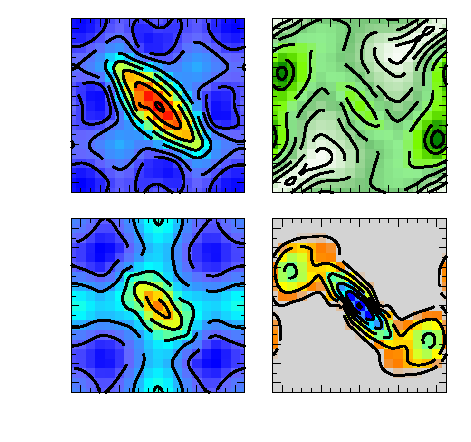
\includegraphics[width={226.00bp},height={212.00bp}]{Figs/Q0_maps}}%
    \gplfronttext
  \end{picture}%
\endgroup
